\chapter{Geometry}
\label{sec:geom}
This section describes the variables and methods used to parameterize
the substructure geometry in \textit{FloatingSE}.  Typically,
substructure designs have fallen into three classical regimes, which are
shown in Figure \ref{fig:archetype}, each of which attains stability
through different physical mechanisms.  A spar derives its stability from a
deep drafted ballast.  A semisubmersible derives its stability from
distributed waterplane area.  A tension leg platform (TLP) uses taut
mooring lines for its stability.

The general configuration of a
spar-type substructure is shown in Figure \ref{fig:diagram}.  The
nomenclature used in Figure \ref{fig:diagram} and \textit{FloatingSE} is
borrowed from the field of naval architecture.  A semisubmersible
configuration would have a similar diagram, but with multiple vertical
columns connected with truss and pontoon elements.
%
\begin{figure}[htb]
  \begin{center}
    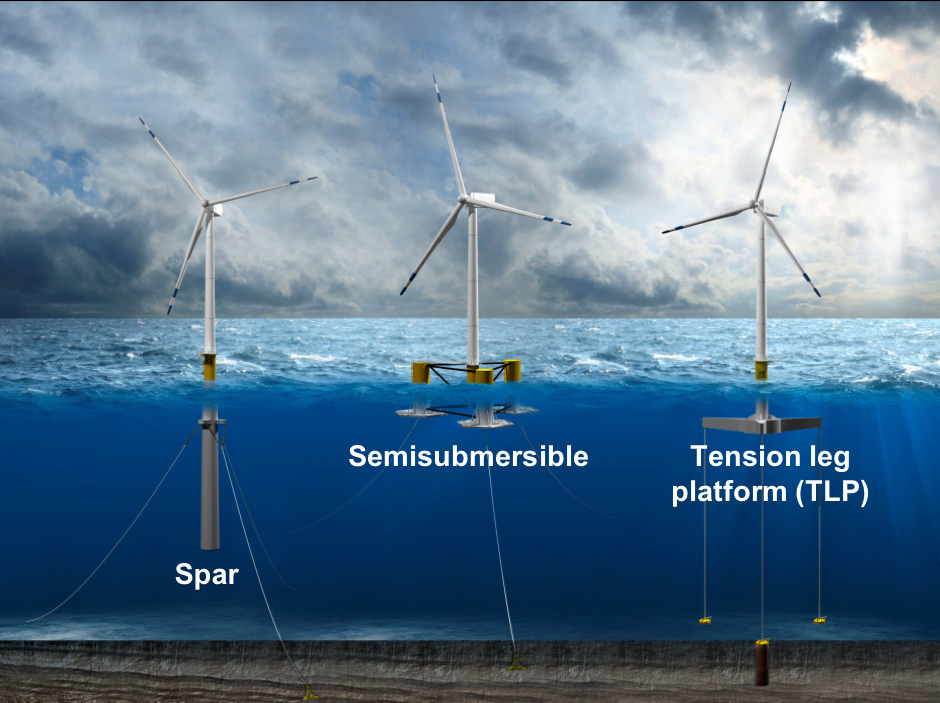
\includegraphics[width=3.75in]{figs/archetypes.pdf}
    \caption{Three classical designs for floating turbine substructures.}
    \label{fig:archetype}
  \end{center}
\end{figure}
%
\begin{figure}[htb]
  \begin{center}
    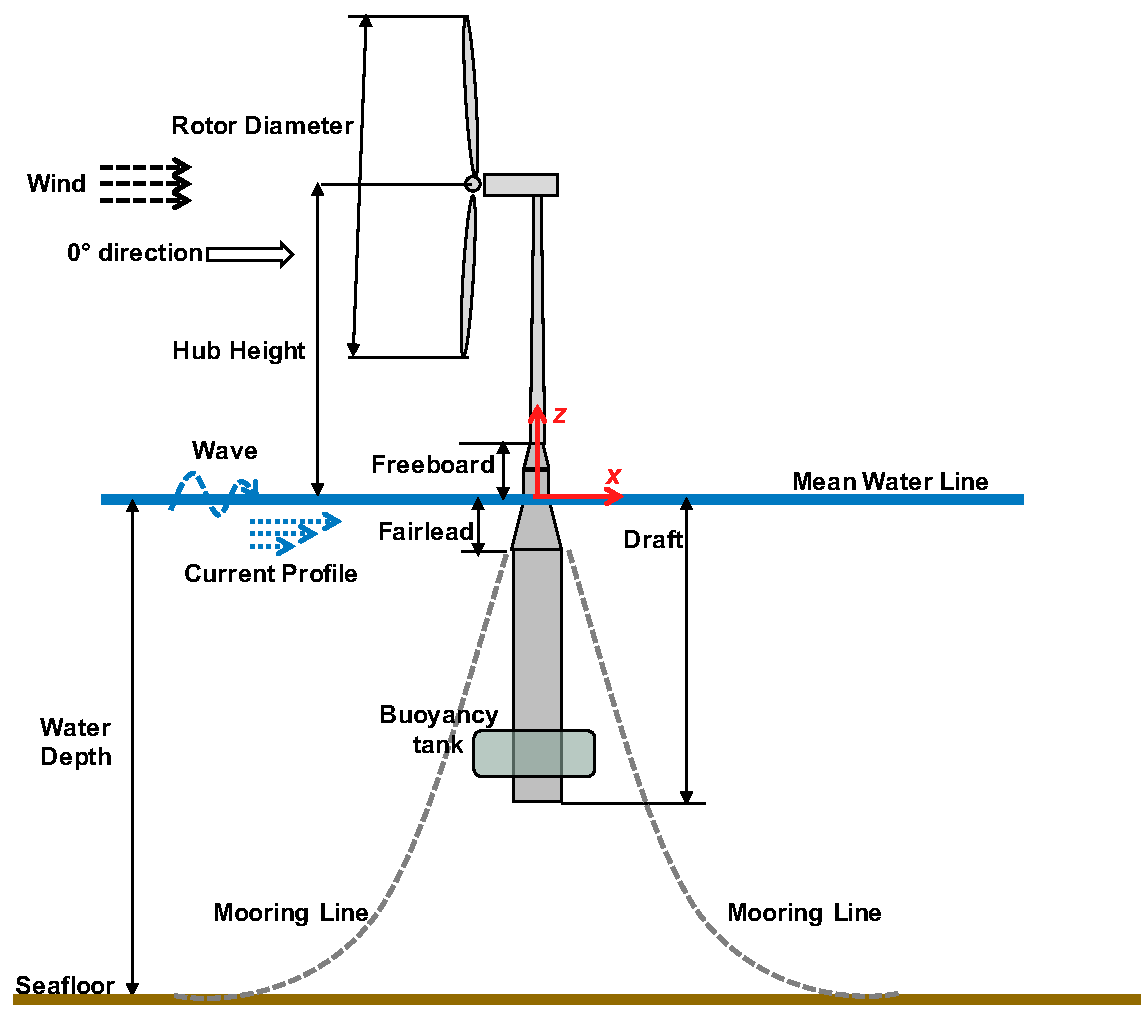
\includegraphics[width=5in]{figs/diagram.pdf}
    \caption{Geometry parameterization with common wind turbine and
      naval architecture conventions.}
    \label{fig:diagram}
  \end{center}
\end{figure}

\section{Discretization}
To allow for varying geometry parameters along the length of
substructure columns, the larger components are divided into sections.
The user may specify the number of overall sections and the geometry of
each section.  Some of the geometry parameters are tied to the nodes
that bracket each section, such as column diameter and wall thickness,
with linear variation between each node.  Other parameters are
considered constant within each section, such as the spacing between
ring stiffeners.  The number of sections should resemble the physical
number of cans or sections used in the manufacturing of the real
article.  The examples provided in \textit{FloatingSE} use 5 sections
for the larger column components.  The user specifies the number of
sections, $n_s$, in the constructor arguments to the \textit{FloatingSE}
group.

For the finite element structural analysis of the substructure, the
discretization of the main columns into a handful of sections is still
too coarse to capture the appropriate dynamics.  Thus, the sectional and
nodal variables are re-sampled at a finer spacing, with each section
sub-divided three times.

\section{Vertical Frustums (Tapered Cylinders)}
A number of typical floating substructure designs, such as the spar or
semisubmersible, contain vertically oriented columns.  These columns can
have a square or circular cross-section, of which only the circular
cross-section (formally a vertical frustum) is currently supported.
These frustums are assumed to be ring-stiffened to support the buckling
loads inherent in a submerged support structure.  The number of columns,
their geometry, and the ring stiffeners are parameterized in the
FloatingSE module according to the diagrams in Figures \ref{fig:diagram}
and \ref{fig:column}.  A ``base'' column is
assumed to centered at $(x=0, y=0)$, directly underneath the turbine
tower (note that off-centered towers are not yet supported).  Other
columns are referred to as ``auxiliary'' columns, and are assumed to be
evenly spread around the base-column.
%
\begin{figure}[htb]
  \begin{subfigure}[b]{0.38\linewidth}
    \centering 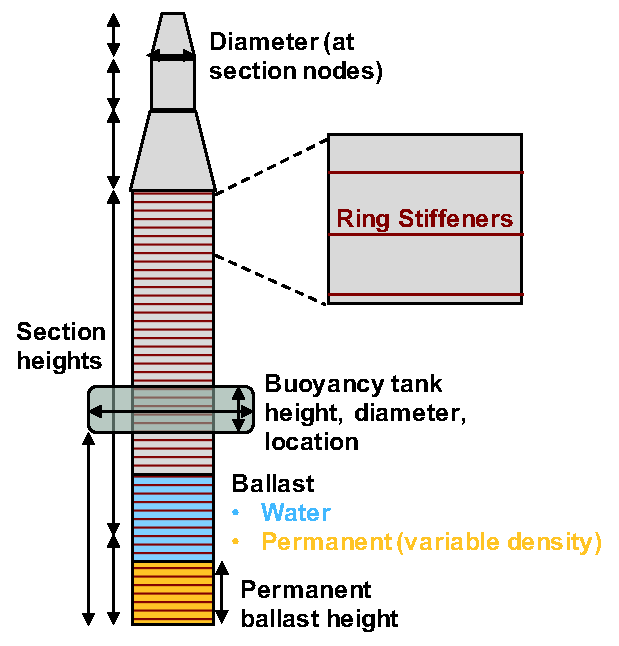
\includegraphics[width=2.2in]{figs/colGeom.pdf}
    \caption{Vertical column of frustums}
  \end{subfigure}
  \begin{subfigure}[b]{0.29\linewidth}
    \centering 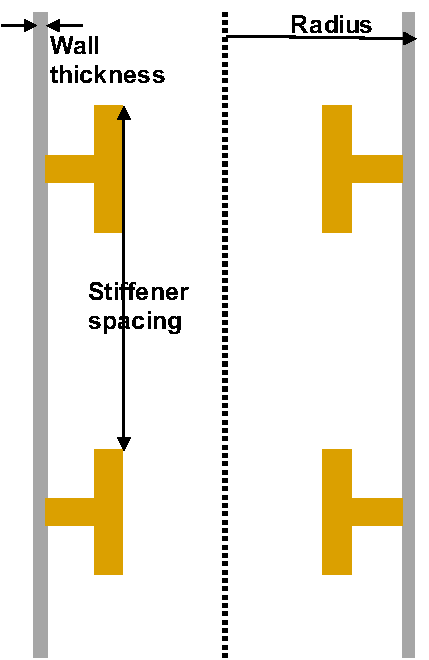
\includegraphics[width=1.8in]{figs/stiffenerCut.pdf}
    \caption{Vertical cross-section}
  \end{subfigure}
  \begin{subfigure}[b]{0.29\linewidth}
    \centering 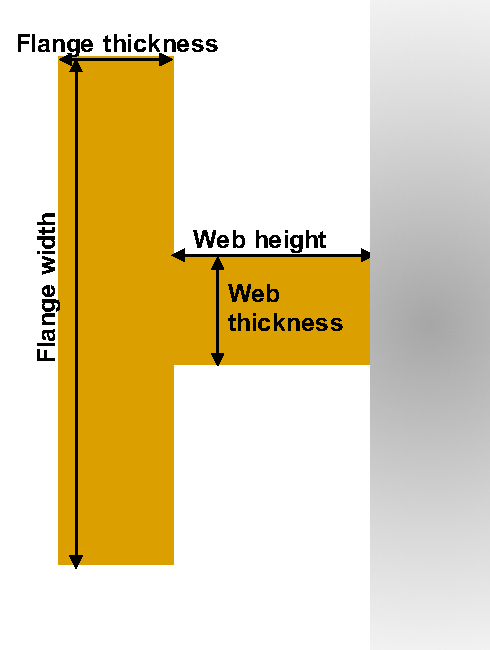
\includegraphics[width=1.8in]{figs/stiffenerZoom.pdf}
    \caption{Ring stiffener geometry}
  \end{subfigure}
  \caption{Vertical frustum geometry parameterization.}
  \label{fig:column}
\end{figure}

\subsection{Geometry}
The variables that set the geometry of the base and auxiliary columns within the
\textit{FloatingSE} Group are listed in Table \ref{tbl:basevar}.  Two
additional variables are also included that describe the placement of
the auxiliary columns within the substructure configuration.
%
\begin{table}[htbp] \begin{center}
    \caption{Variables specifying the base column geometry within \textit{FloatingSE}.}
    \label{tbl:basevar}
{\footnotesize
  \begin{tabular}{ l l c l } \hline
    \textbf{Variable} & \textbf{Type} & \textbf{Units} & \textbf{Description} \\
    \mytt{base\_section\_height} & Float array ($n_s$) & $m$& Height of each section \\
    \mytt{base\_outer\_diameter} & Float array ($n_s+1$) & $m$&Diameter at each section node (linear lofting between) \\
    \mytt{base\_wall\_thickness} & Float array ($n_s+1$) & $m$&Wall thickness at each section node (linear lofting between) \\
    \mytt{base\_freeboard} & Float scalar & $m$&Design height above waterline \\
    \mytt{auxiliary\_section\_height} & Float array ($n_s$) & $m$& Height of each section \\
    \mytt{auxiliary\_outer\_diameter} & Float array ($n_s+1$) & $m$&Diameter at each section node (linear lofting between) \\
    \mytt{auxiliary\_wall\_thickness} & Float array ($n_s+1$) & $m$&Wall thickness at each section node (linear lofting between) \\
    \mytt{auxiliary\_freeboard} & Float scalar & $m$&Design height above waterline \\
    \mytt{number\_of\_auxiliary\_columns} & Integer scalar && Number of auxiliary columns in substructure (for spar set to 0)\\
    \mytt{radius\_to\_auxiliary\_column} & Float scalar &$m$& Centerline of base column to centerline of auxiliary column\\
  \hline \end{tabular}
}
\end{center} \end{table}

\subsection{Stiffeners}
The ring stiffener geometry is depicted in Figure \ref{fig:column}b--c
with geometry variables listed in Table \ref{tbl:stiffvar}
%
\begin{table}[htbp] \begin{center}
    \caption{Variables specifying the stiffener geometry within \textit{FloatingSE}.}
    \label{tbl:stiffvar}
{\footnotesize
  \begin{tabular}{ l l c l } \hline
    \textbf{Variable} & \textbf{Type} & \textbf{Units} & \textbf{Description} \\
    \mytt{base\_stiffener\_web\_height} & Float array ($n_s$) &$m$& Stiffener web height for each section \\
    \mytt{base\_stiffener\_web\_thickness} & Float array ($n_s$) &$m$& Stiffener web thickness for each section\\
    \mytt{base\_stiffener\_flange\_width} & Float array ($n_s$) &$m$& Stiffener flange width for each section\\
    \mytt{base\_stiffener\_flange\_thickness} & Float array ($n_s$) &$m$& Stiffener flange thickness for each section\\
    \mytt{base\_stiffener\_spacing} & Float array ($n_s$) &$m$& Stiffener spacing for each section\\
  \hline \end{tabular}
}
\end{center} \end{table}

\subsection{Material Properties}
The material of the vertical columns is currently assumed to uniformly
be ASTM 992 steel.  Future developments will include the option to
select one of multiple material options for each section in each
cylinder.  Currently, to globally change to a different material, use
the variables listed in Table \ref{tbl:materialvar}.
%
\begin{table}[htbp] \begin{center}
    \caption{Variables specifying the material properties within \textit{FloatingSE}.}
    \label{tbl:materialvar}
{\footnotesize
  \begin{tabular}{ l l c l } \hline
    \textbf{Variable} & \textbf{Type} & \textbf{Units} & \textbf{Description} \\
    \mytt{material\_density} & Float scalar & $kg/m^3$& Mass density (assumed steel) \\
    \mytt{E} & Float scalar & $N/m^2$& Young's modulus (of elasticity) \\
    \mytt{G} & Float scalar & $N/m^2$& Shear modulus \\
    \mytt{yield\_stress} & Float scalar & $N/m^2$& Elastic yield stress \\
    \mytt{nu} & Float scalar && Poisson's ratio ($\nu$)\\
  \hline \end{tabular}
}
\end{center} \end{table}

\subsection{Ballast}
Substructure columns with long drafts can enhance stability by placing heavy
ballast at their keel (bottom point).  Bulkheads between column sections
help to keep the ballast in place, or serve as dividers between other
section roles.  The variables that govern the implementation of the
permanent ballast and bulkhead nodes are listed in Table
\ref{tbl:ballastvar}. Variable ballast, as opposed to permanent ballast, is water that is
added or removed above the permanent ballast to achieve neutral buoyancy as the
operating conditions of the turbine change.  A discussion of variable
balance in the model is found in Section \ref{sec:static}.
%
\begin{table}[htbp] \begin{center}
    \caption{Variables specifying the ballast and bulkheads within \textit{FloatingSE}.}
    \label{tbl:ballastvar}
{\footnotesize
  \begin{tabular}{ l l c l } \hline
    \textbf{Variable} & \textbf{Type} & \textbf{Units} & \textbf{Description} \\
    \mytt{permanent\_ballast\_density} & Float scalar & $kg/m^3$& Mass density of ballast material \\
    \mytt{base\_permanent\_ballast\_height} & Float scalar & $m$& Height above keel for permanent ballast \\
    \mytt{base\_bulkhead\_nodes} & Boolean list ($n_s+1$) && Locations of internal bulkheads at section interfaces\\
    \mytt{auxiliary\_permanent\_ballast\_height} & Float scalar & $m$& Height above keel for permanent ballast \\
    \mytt{auxiliary\_bulkhead\_nodes} & Boolean list ($n_s+1$) && Locations of internal bulkheads at section interfaces\\
  \hline \end{tabular}
}
\end{center} \end{table}


\subsection{Buoyancy Tanks (and Heave Plates)}
Buoyancy tanks are modeled as a collar around the column and are
not subject the same taper or connectivity constraints as the frustum
sections.  They therefore offer added buoyancy without incurring as much
structural mass or cost.  Additionally, they can also serve to augment
the heave added mass like a heave plate.  The variables that govern
their configuration are listed in Table \ref{tbl:buoyheave}.  In
addition to their diameter and height, the user can adjust the location
of the buoyancy tank from $0$, the column base, to $1$, the top of
column. Buoyancy tanks can be added to either the base and/or auxiliary columns.
%
\begin{table}[htbp] \begin{center}
    \caption{Variables specifying the buoyancy tank geometry within \textit{FloatingSE}.}
    \label{tbl:ballastvar}
{\footnotesize
  \begin{tabular}{ l l c l } \hline
    \textbf{Variable} & \textbf{Type} & \textbf{Units} & \textbf{Description} \\
    \mytt{base\_buoyancy\_heave\_box\_diameter} & Float scalar & $m$& Diameter of buoyancy tank / heave plate on base column\\
    \mytt{base\_buoyancy\_heave\_box\_height} & Float scalar & $m$& Height of buoyancy tank / heave plate on base column\\
    \mytt{base\_buoyancy\_heave\_box\_location} & Float scalar & & Location of buoyancy tank along base column (0 for bottom, 1 for top)\\
    \mytt{auxiliary\_buoyancy\_heave\_box\_diameter} & Float scalar & $m$& Diameter of buoyancy tank / heave plate on auxiliary column\\
    \mytt{auxiliary\_buoyancy\_heave\_box\_height} & Float scalar & $m$& Height of buoyancy tank / heave plate on auxiliary column\\
    \mytt{auxiliary\_buoyancy\_heave\_box\_location} & Float scalar & & Location of buoyancy tank along auxliary column (0 for bottom, 1 for top)\\
  \hline \end{tabular}
}
\end{center} \end{table}

\section{Pontoons and Support Structure}
Many substructure designs include the use of pontoons that form a truss
to connect the different components, usually columns, together.  In this
model, all of the pontoons are assumed to have the identical thin-walled
tube cross section and made of the same material as the rest of the
substructure.  The truss configuration and the parameterization of the
pontoon elements is based on the members shown in Figure
\ref{fig:pontoon}.  The members are broken out into the upper and lower
rings connecting the auxiliary columns, the upper and lower
base-to-auxiliary connections, the lower-base to upper-auxiliary cross
members, and the V-shaped cross members between auxiliary columns.  The
variables that drive this parameterization are listed in Table
\ref{tbl:trussvar}.
%
\begin{figure}[htb]
  \begin{center}
    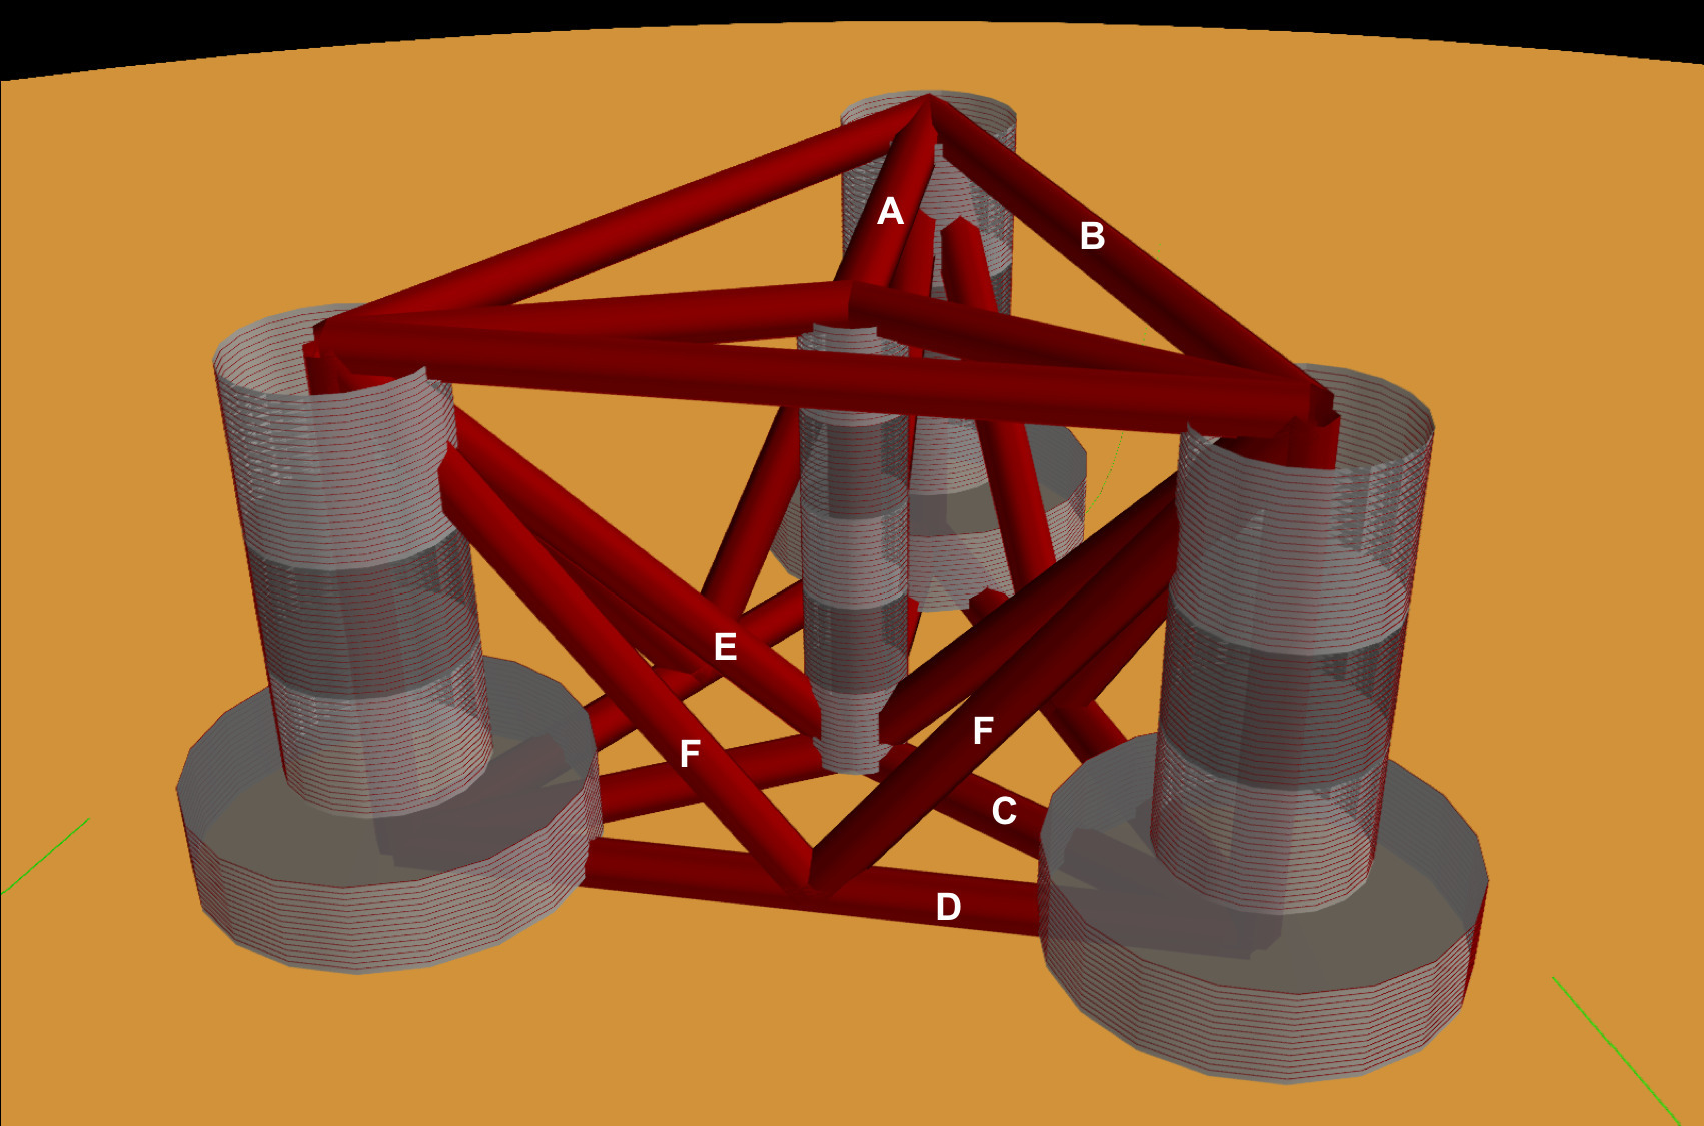
\includegraphics[width=4.5in]{figs/semi.pdf}
    \caption{Parameterization of truss elements in substructure.}
    \label{fig:pontoon}
  \end{center}
\end{figure}
%
\begin{table}[htbp] \begin{center}
    \caption{Variables specifying the pontoon and truss geometry within \textit{FloatingSE}.}
    \label{tbl:trussvar}
{\footnotesize
  \begin{tabular}{ l l c c l } \hline
    \textbf{Variable} & \textbf{Type} & \textbf{Figure \ref{fig:pontoon}} & \textbf{Units} & \textbf{Description} \\
    \mytt{pontoon\_outer\_diameter} & Float scalar & & $m$& Diameter of all pontoon/truss elements \\
    \mytt{pontoon\_wall\_thickness} & Float scalar & & $m$& Thickness of all pontoon/truss elements \\
    \mytt{base\_pontoon\_attach\_lower} & Float scalar & & $m$& Lower z-coordinate on base where truss attaches \\
    \mytt{base\_pontoon\_attach\_upper} & Float scalar & & $m$& Upper z-coordinate on base where truss attaches \\
    \mytt{upper\_attachment\_pontoons} & Boolean & A && Upper base-to-auxiliary connecting pontoons\\
    \mytt{lower\_attachment\_pontoons} & Boolean & C && Lower base-to-auxiliary connecting pontoons\\
    \mytt{cross\_attachment\_pontoons} & Boolean & E && Lower-Upper base-to-auxiliary connecting cross braces\\
    \mytt{upper\_ring\_pontoons} & Boolean & B && Upper ring of pontoons connecting auxiliary columns\\
    \mytt{lower\_ring\_pontoons} & Boolean & D && Lower ring of pontoons connecting auxiliary columns\\
    \mytt{outer\_cross\_pontoons} & Boolean & F && Auxiliary ring connecting V-cross braces\\
  \hline \end{tabular}
}
\end{center} \end{table}


\section{Mooring Lines}
The mooring system is described by the number of lines, their geometry,
and their interface to the substructure.  The mooring diameter is
specified directly and determines the breaking load and stiffness of the
chain (via correlation, described in Section \ref{sec:theory}).  The
mooring lines attach to the substructure at the ``fairlead'' distance
below the water plane, as shown in Figure \ref{fig:diagram}.  The lines
can attach directly to a substructure column or at a some offset from
the outer surface.  Note that bridle connections are not yet
implemented.  The mooring lines attach to the sea floor at a variable
distance from the substructure centerline and their total length is
also specified by the user.

By default, the mooring system is assumed to use a steel chain with drag
embedment anchors. Other mooring available for selection are nylon,
polyester, steel wire rope (IWRC) and fiber-core wire rope.  The only
alternative anchor type is currently suction pile anchors, but there are
plans to include gravity anchors as well.  The standard configuration
for TLPs is the use of taut nylon mooring lines with suction-pile
anchors.  The variables that control the mooring system properties are
listed in Table \ref{tbl:moorvar}.

\begin{table}[htbp] \begin{center}
    \caption{Variables specifying the mooring system within \textit{FloatingSE}.}
    \label{tbl:moorvar}
{\footnotesize
  \begin{tabular}{ l l c l } \hline
    \textbf{Variable} & \textbf{Type} & \textbf{Units} & \textbf{Description} \\
    \mytt{number\_of\_mooring\_connections} & Integer scalar && Number of mooring connection points evenly spaced around structure\\
    \mytt{mooring\_lines\_per\_connection} & Integer scalar && Number of mooring lines at each connection point\\
    \mytt{mooring\_diameter} & Float scalar & $m$& Diameter of mooring line/chain \\
    \mytt{mooring\_line\_length} & Float scalar &$m$& Total unstretched line length of mooring line\\
    \mytt{fairlead} & Float scalar & $m$& Distance below waterline for attachment \\
    \mytt{fairlead\_offset\_from\_shell} & Float scalar & $m$ & Offset from shell surface for mooring attachment \\
    \mytt{anchor\_radius} & Float scalar & $m$& Distance from centerline to sea floor landing \\
    \mytt{mooring\_type} & Enumerated & & Options are CHAIN, NYLON, POLYESTER, FIBER, or IWRC\\
    \mytt{anchor\_type} & Enumerated & & Options are SUCTIONPILE or DRAGEMBEDMENT\\
  \hline \end{tabular}
}
\end{center} \end{table}


\section{Mass and Cost Scaling}
The mass of all components in the modeled substructure is captured
through calculation of each components' volume and multiplying by its material
density.  This applies to the frustum shells, the ring stiffeners, the
permanent and water ballast, the pontoons, and the mooring lines.
However, the model also acknowledges that the modeled substructure is
merely an approximation of an actual substructure and various secondary
elements are not captured.  These include ladders, walkways, handles,
finishing, paint, wiring, etc.  To account for these features en masse,
multipliers of component masses are offered as parameters for the user,
which are listed in Table \ref{tbl:massvar}.

Also included in Table \ref{tbl:massvar} are cost multipliers.  These variables
scale substructure component mass totals by an empirically determined
value (with units of cost per unit mass) to arrive at a substructure
cost.  This determination is challenging due to the proprietary nature
of commercial cost data.

\begin{table}[htbp] \begin{center}
    \caption{Variables specifying the mass and cost scaling within \textit{FloatingSE}.}
    \label{tbl:massvar}
{\footnotesize
  \begin{tabular}{ l l c l } \hline
    \textbf{Variable} & \textbf{Type} & \textbf{Description} \\
    \mytt{bulkhead\_mass\_factor}     & Float scalar     && Scaling for unaccounted bulkhead mass\\
    \mytt{ring\_mass\_factor}         & Float scalar     && Scaling for unaccounted stiffener mass\\
    \mytt{shell\_mass\_factor}        & Float scalar     && Scaling for unaccounted shell mass\\
    \mytt{column\_mass\_factor}       & Float scalar    && Scaling for unaccounted column mass\\
    \mytt{outfitting\_mass\_fraction} & Float scalar    && Fraction of additional outfitting mass for each column\\
    \mytt{ballast\_cost\_rate}        & Float scalar   & $USD/kg$& Cost factor for ballast mass \\
    \mytt{tapered\_col\_cost\_rate}    & Float scalar  & $USD/kg$& Cost factor for column mass \\
    \mytt{outfitting\_cost\_rate}     & Float scalar  & $USD/kg$& Cost factor for outfitting mass \\
    \mytt{mooring\_cost\_rate}        & Float scalar     & $USD/kg$& Cost factor for mooring mass \\
    \mytt{pontoon\_cost\_rate}        & Float scalar   & $USD/kg$& Cost factor for pontoons \\
  \hline \end{tabular}
}
\end{center} \end{table}
